\documentclass[12pt]{article}
\usepackage[top=1in,bottom=1in,left=1in,right=1in]{geometry}
\usepackage{alltt}
\usepackage{array}	
\usepackage{graphicx}
\usepackage{tabularx}
\usepackage{verbatim}
\usepackage{setspace}
\usepackage{listings}
\usepackage{amssymb,amsmath, amsthm}

\title{SOEN331: Introduction to Formal Methods\\for Software Engineering\\
Assignment 1 on extended finite state machines}
\author{Tarek Ait Hamouda (40044119), Abhijit Gupta (40066502),\\ 
Ethel Narra Pangan (40061530)}
\date{\today}

\begin{document}
\begin{spacing}{1.5}

\maketitle

\section{Room temperature control formal specification}

\noindent The EFSM of the room temperature control is the tuple $S = (Q, \Sigma_1, \Sigma_2, q_0, V, \Lambda)$, where
\noindent $Q = \{idle, warm up, configuration\}$\\
\noindent $\Sigma_1 = \{shut off, setup, interrupt, after(3min), after(2min), after~1~min~inactive, cancel, completed\}$\\
\noindent $\Sigma_2 = \{fan~on, fan~off, furnace~on, furnace~off, prolonged~beep~sound, double~beep~sound\}$\\
\noindent $q_0: idle$\\
\noindent $V: \{C, T, D, Tf\}$\\
\noindent $\Lambda$: Transition specifications\\
\indent 1. $\rightarrow idle$\\
\indent 2. $idle \xrightarrow {\text { shut off/ (fan off; furnace off)}} off$\\
\indent 3. $idle \xrightarrow {\text { after(2min)[C $\geq$ D]}} idle$\\
\indent 4. $idle \xrightarrow {\text { after(2min)[C $\leq$ D-1] / (fan off; furnace on)}} warm~up$\\
\indent 5. $idle \xrightarrow {\text {setup}/(beep sound ; led light switch on)} configuration$\\
\indent 6. $warm~up \xrightarrow {\text { after(3min)[T.F $<$ D+1] }} warm~up$\\
\indent 7. $warm~up \xrightarrow {\text { after(3min)[T.F $\geq$ D+1]/(fan on; furnace off; click sound) }} idle$\\
\indent 8. $warm~up \xrightarrow {\text { interrupt/furnace off }} configuration$\\
\indent 9. $configuration \xrightarrow {\text { after 1 min inactive / led light switch off }} idle$\\
\indent 10. $configuration \xrightarrow {\text { cancel/(prolonged beep sound;led light switch off) }} idle$\\
\indent 11. $configuration \xrightarrow {\text { completed/(double beep sound; led light switch off) }} idle$\\
\noindent The UML state diagram is shown in Figure~\ref{fig:system-fig}.\\\\

\noindent The EFSM of the configuration is the tuple $S = (Q, \Sigma_1, \Sigma_2, q_0, V, \Lambda)$, where\\
\noindent $Q = \{input, add, override, exit\}$\\
\noindent $\Sigma_1 = \{after(1 min)\}$\\
\noindent $\Sigma_2 = \{\}$\\
\noindent $q_0: input$\\
\noindent $V: triplet$\\
\noindent $\Lambda$: Transition specifications\\
\indent 1. $\rightarrow input$\\
\indent 2. $input \xrightarrow {\text { register[triplet does not exist]}} add$\\
\indent 3. $input \xrightarrow {\text { register[triplet exist]}} override$\\
\indent 4. $add \xrightarrow {\text {repeat}} input$\\
\indent 5. $override \xrightarrow {\text {repeat}} input$\\

\noindent The UML state diagram is shown in Figure~\ref{fig:configuration-fig}.

\newpage

\section{UML state diagrams}

\begin{figure}[h!]
	\centering
		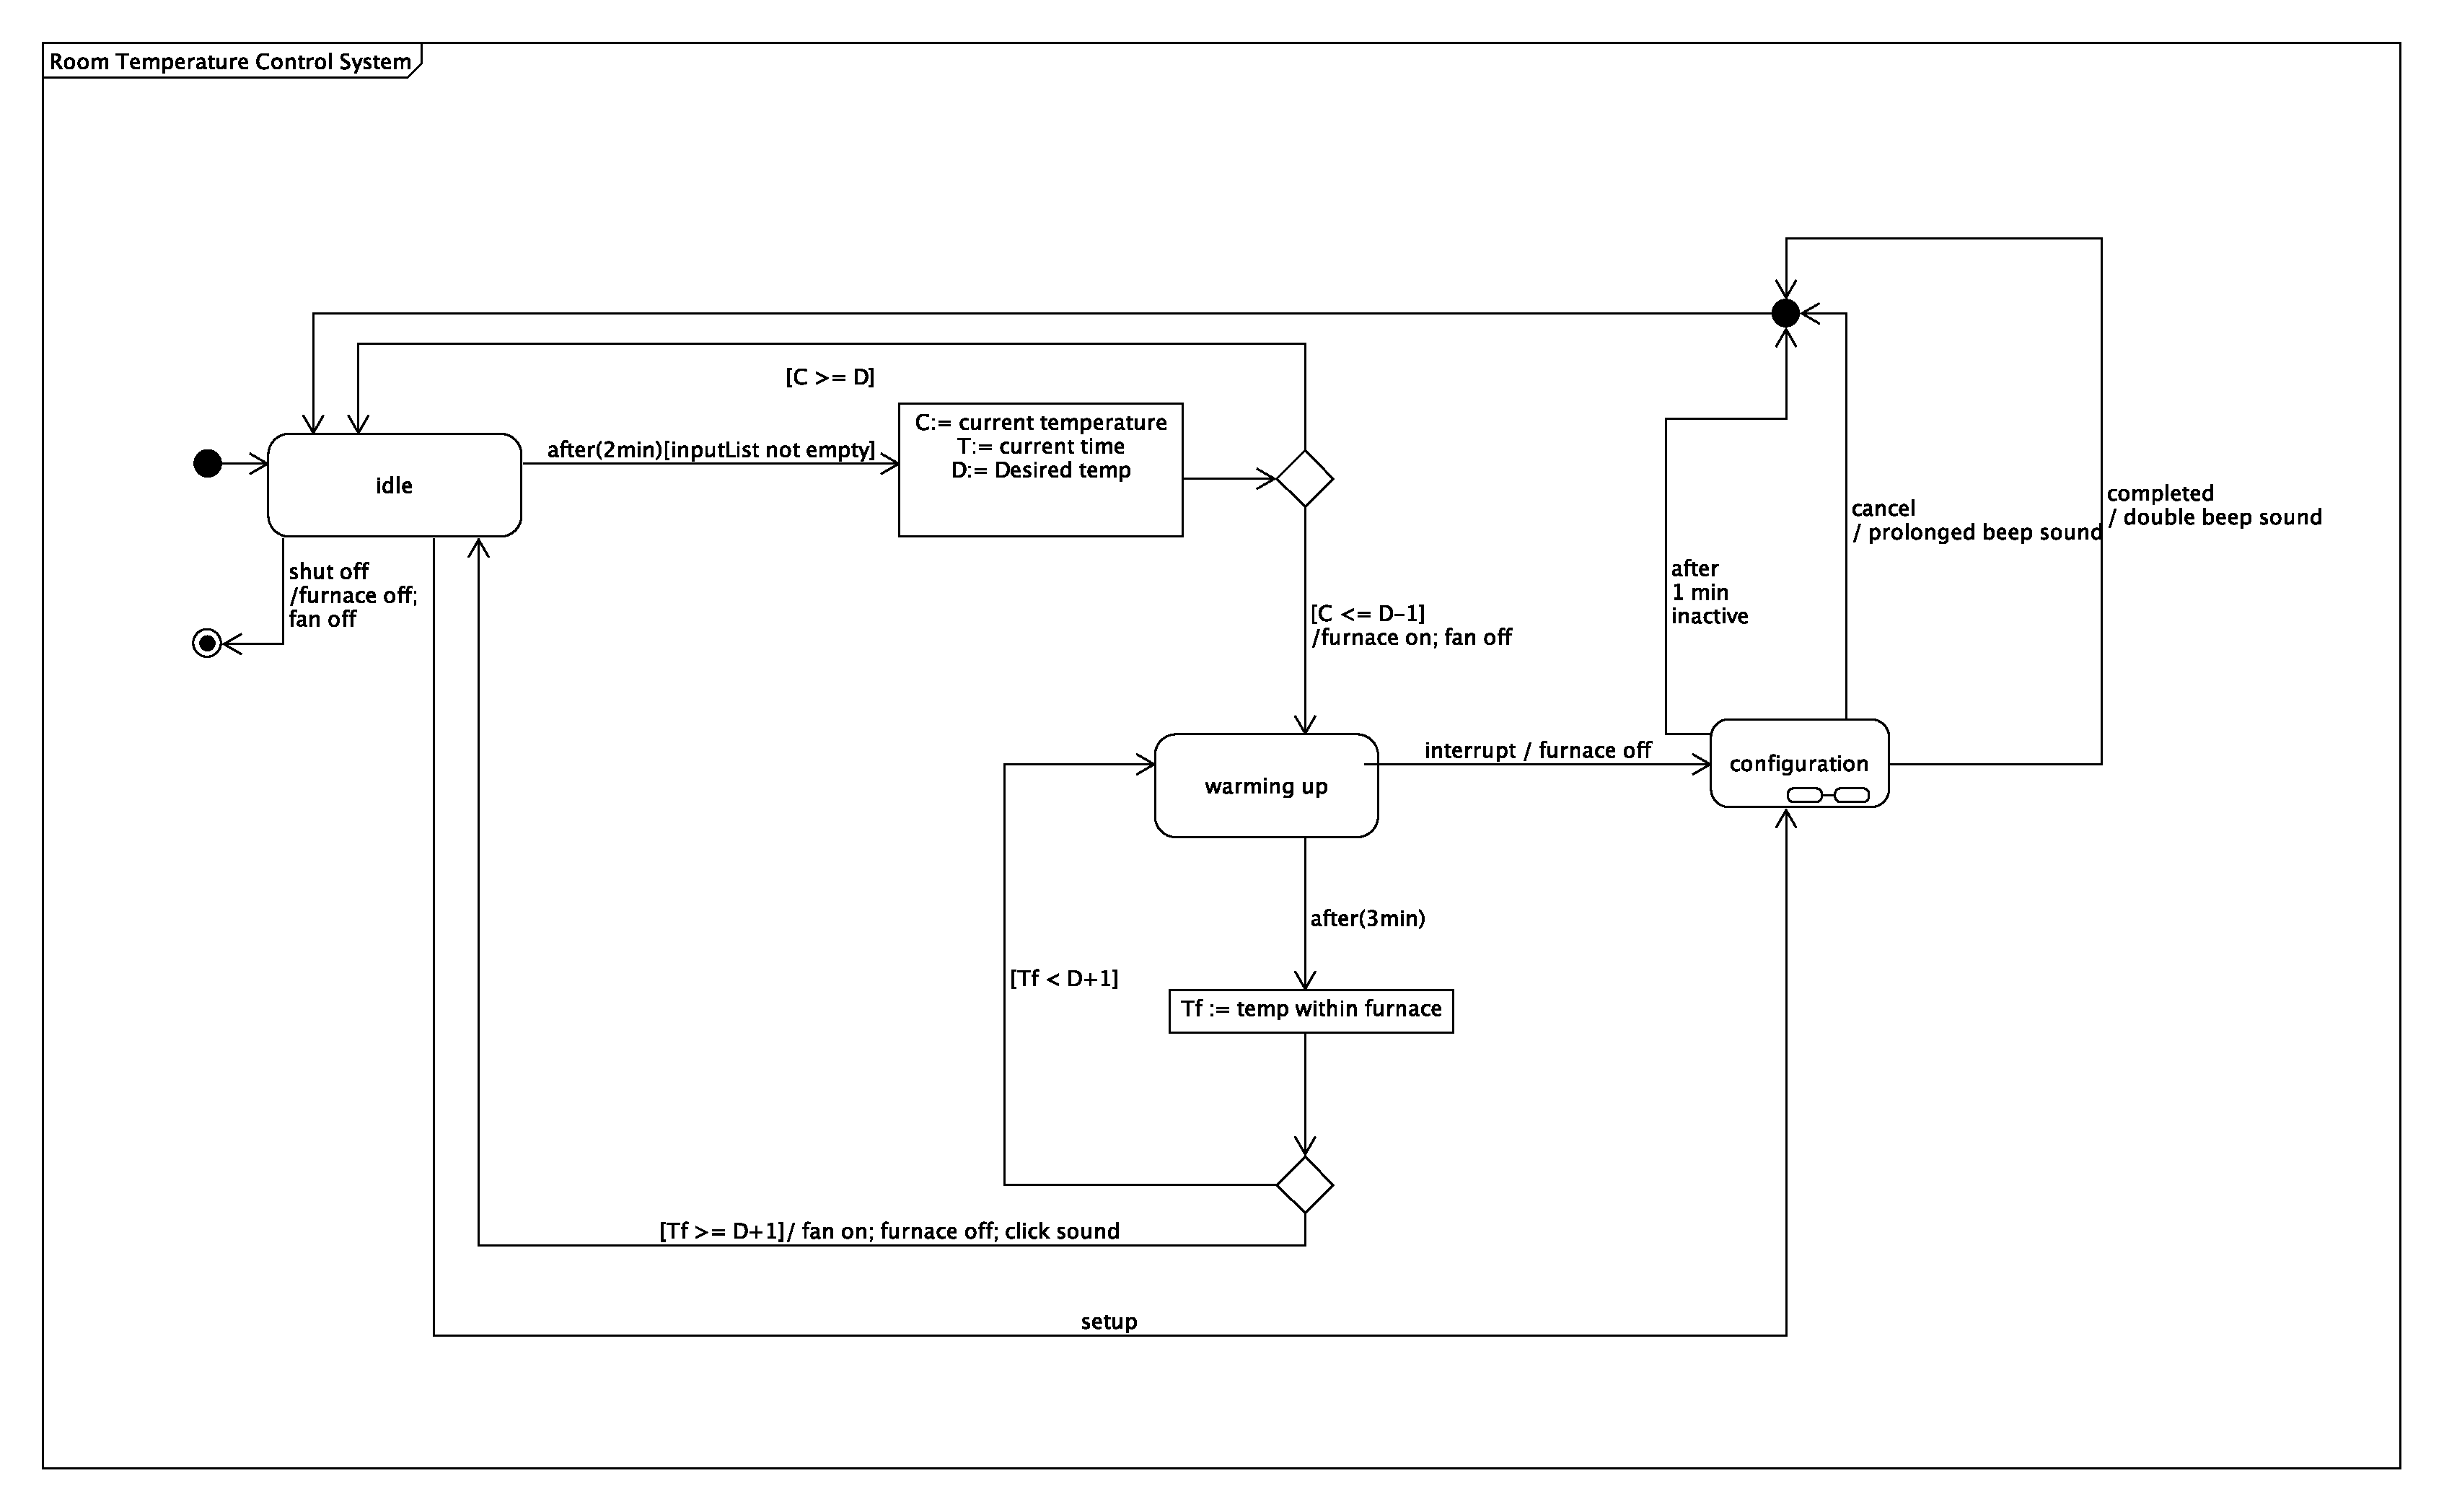
\includegraphics[width=0.8\textwidth]{./figures/eps/SystemEFSM.eps}
		  \caption{Room Temperature Control System UML State Diagram}
  \label{fig:system-fig}
\end{figure}

\begin{figure}[h!]
	\centering
		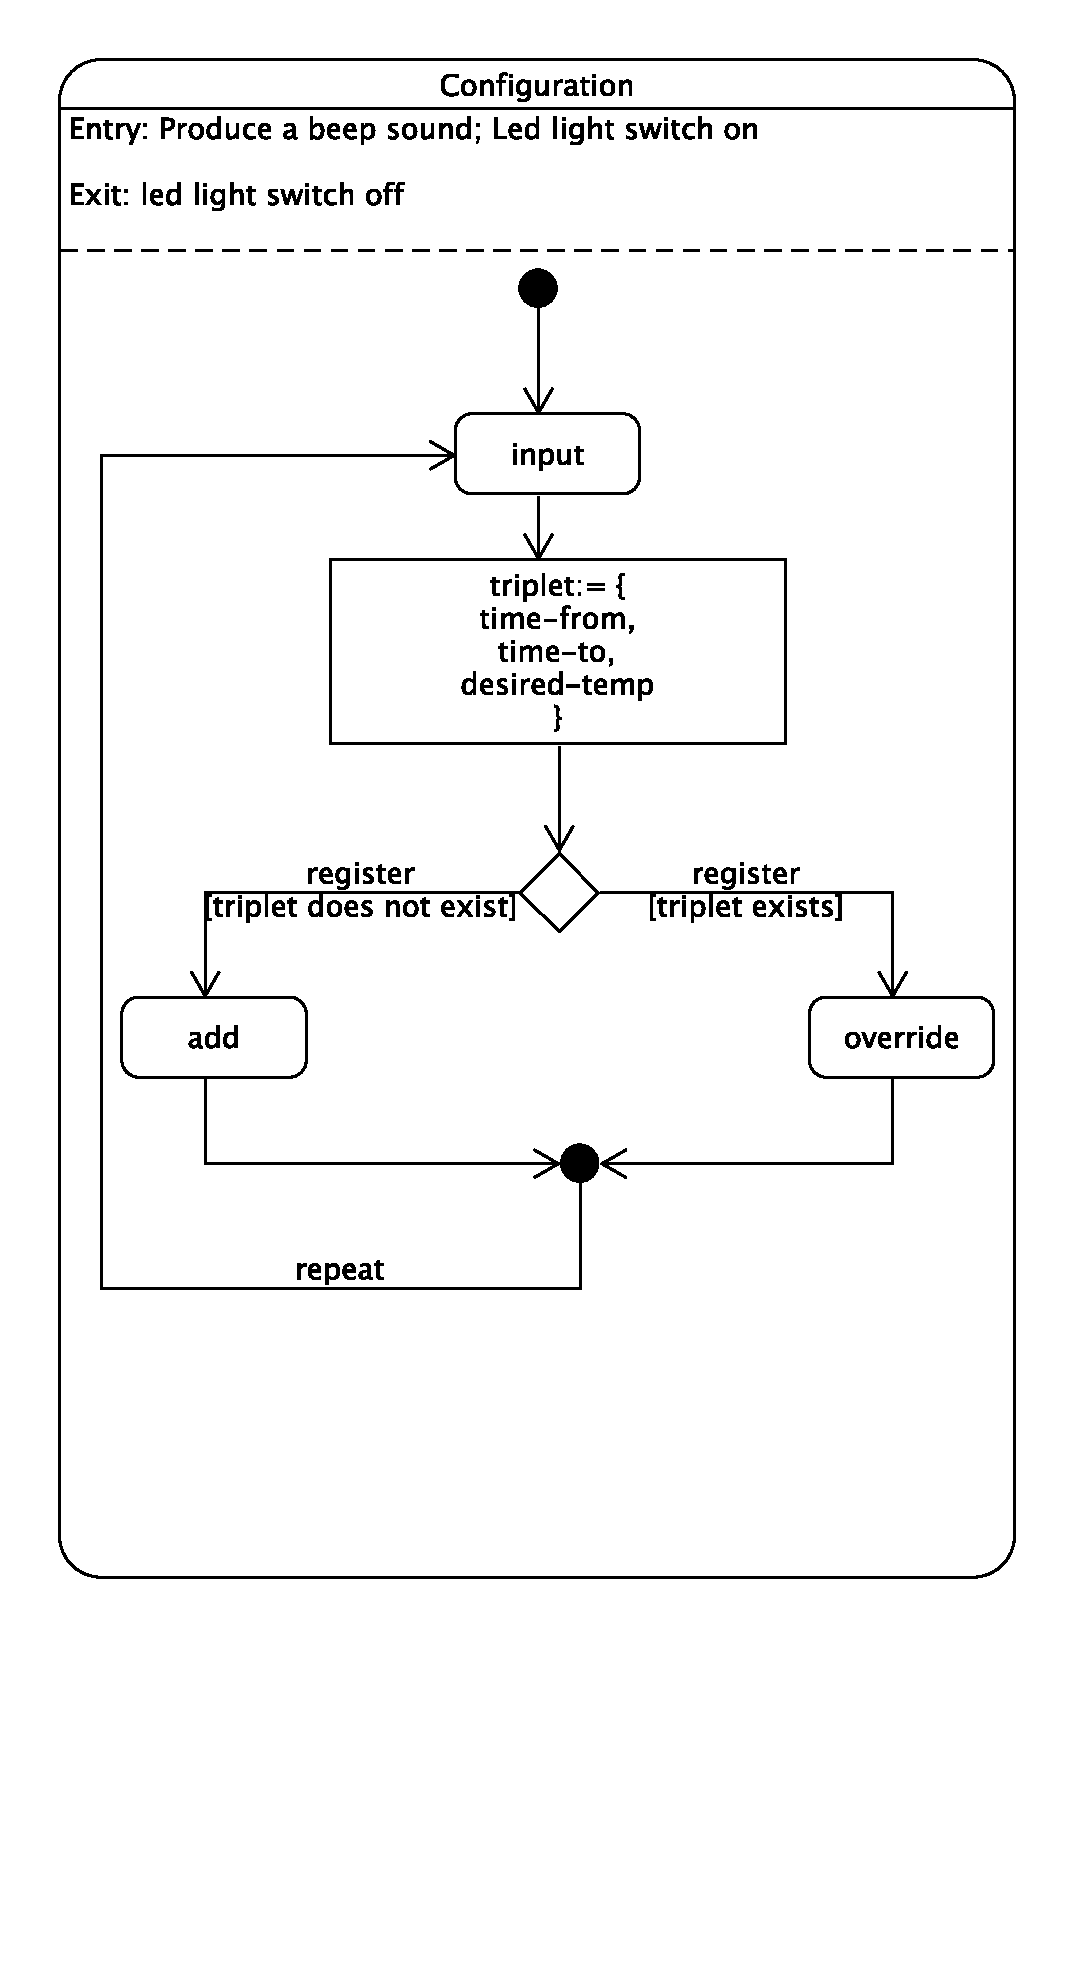
\includegraphics[trim ={0 200pt 0 200pt }, width=0.8\textwidth]{./figures/eps/configurationEFSM.eps}
		  \caption{Configuration UML State Diagram}
  \label{fig:configuration-fig}
\end{figure}

\end{spacing}
\end{document}
